% D.21 垂径定理：⊙O 半径 5，弦 AB=8，OM⊥AB 于 M，P 在 AB 上 AP=2
\documentclass[tikz,border=4pt]{standalone}
\usepackage{ctex}
\usepackage{amsmath}
\usetikzlibrary{calc}
\begin{document}
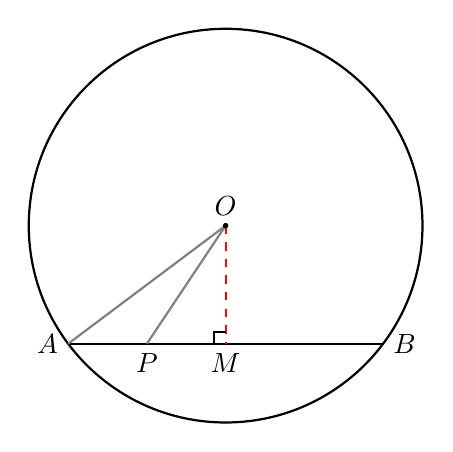
\begin{tikzpicture}[scale=0.5, thick]
  \coordinate (O) at (0, 0);
  \draw (O) circle (5);
  % 取弦 AB 水平、AB=8，则 OM=3，M=(0,-3)，A=(-4,-3)，B=(4,-3)
  \coordinate (A) at (-4, -3);
  \coordinate (B) at ( 4, -3);
  \coordinate (M) at ( 0, -3);
  \coordinate (P) at (-2, -3);  % AP=2

  \draw (A) -- (B);
  \draw[red, dashed] (O) -- (M);
  \draw[gray] (O) -- (A);
  \draw[gray] (O) -- (P);
  % 直角符号
  \draw (-0.3,-3) -- (-0.3,-2.7) -- (0,-2.7);

  \fill (O) circle (2pt);
  \node[above] at (O) {$O$};
  \node[left]  at (A) {$A$};
  \node[right] at (B) {$B$};
  \node[below] at (M) {$M$};
  \node[below] at (P) {$P$};
\end{tikzpicture}
\end{document}
